% !TeX root = ../note.tex
\section{Общие положения}
\subsection{Назначение документа}
В настоящем документе приводится полный набор требований системе, необходимых для реализации.

\subsection{Цели создания проекта}
Проект создается в рамках курса лабораторных работ по предмету Технологии Разработки Программного обеспечения (ТРПО).

\subsection{Краткое описание проекта}
Проект представляет из себя систему для обработки и хранения данных сотового оператора.
Назначение проекта:
\begin{itemize}
    \item создание системы для обработки информации, поступающей с back-end серверов оператора
    \item хранение всех данных компании
    \item предоставление back-end разработчикам API, покрывающего все основные сценарии использования системы
\end{itemize}

\begin{figure}[H]
    \centering
    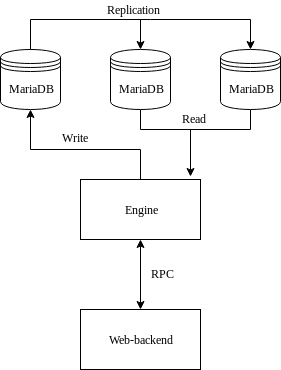
\includegraphics[scale=0.8]{pics/general.png}
    \caption{Примерная схема работы}
\end{figure}

\newpage
